\documentclass[11.5pt]{exam}
\usepackage{ragged2e}
\usepackage{graphicx}
\usepackage{microtype}
\usepackage{multicol}
\usepackage{float}
\usepackage{tabularray}
\usepackage{xcolor}

\pagestyle{head}
\begin{document}
\textbf{Appendix A – Closed-Ended Assessment}

\justifying
Content Assessment - Human Heart \hspace{3.5in} Pre Post
\RaggedRight
\begin{questions}
\question The Human Heart has how many chambers?

\begin{oneparchoices}
 \choice One
 \choice Two
 \choice Three
 \choice Four
\end{oneparchoices}

\question Look at the following pictures. Which picture shows the correct orientation of the heart if you placed it in the chest of the skeleton (shown right)?”

\begin{oneparchoices}
 \choice 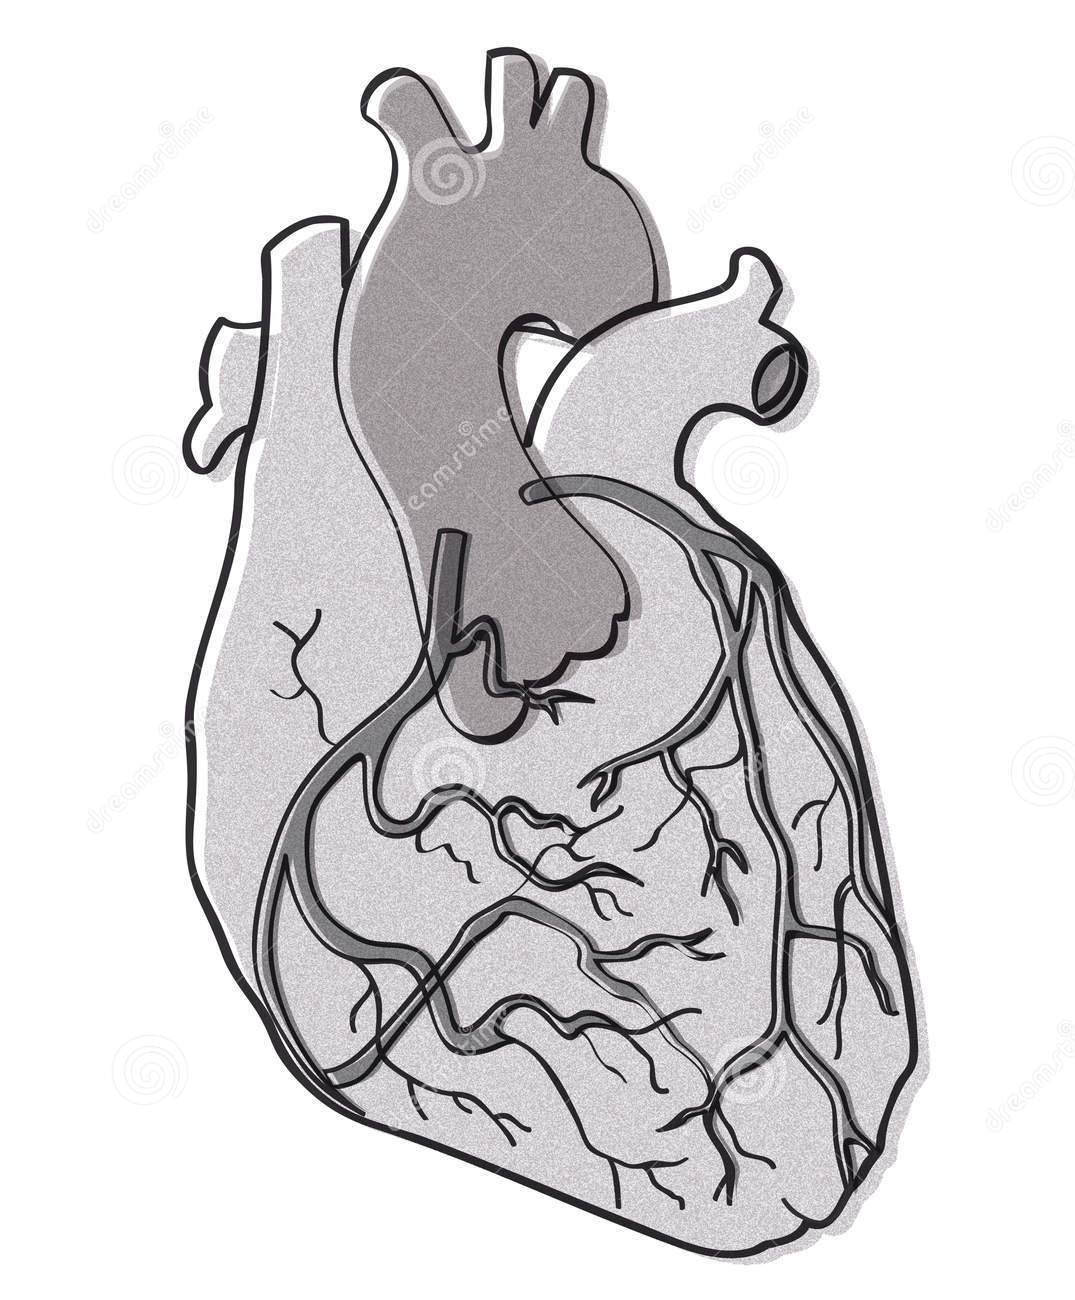
\includegraphics[width=2cm]{quiz/heartA.png}
 \choice 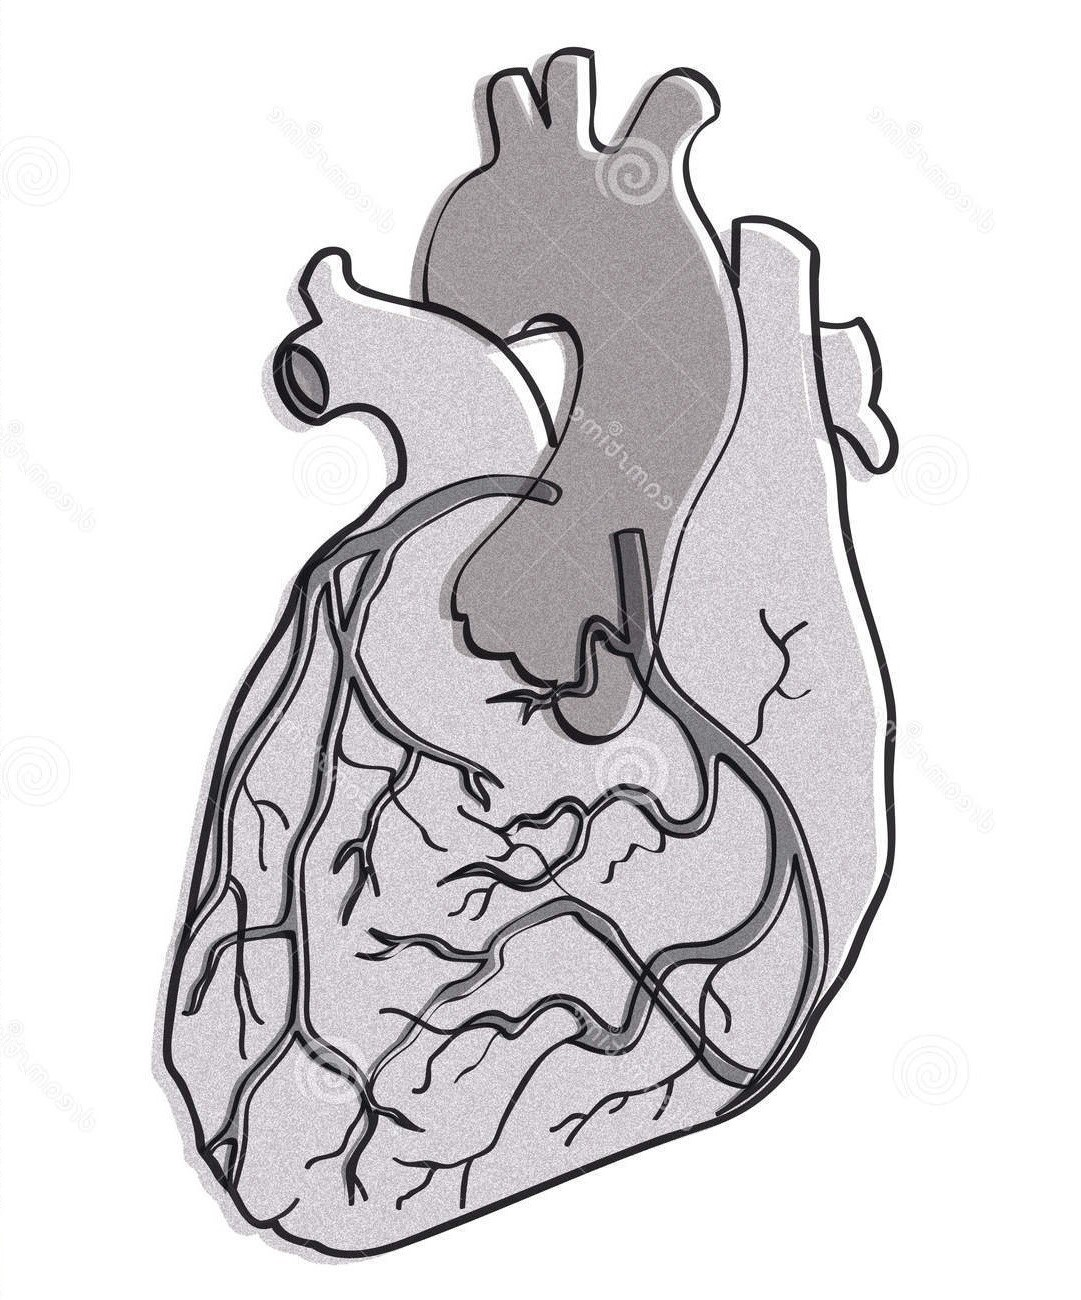
\includegraphics[width=2cm]{quiz/heartB.jpg}
 \choice 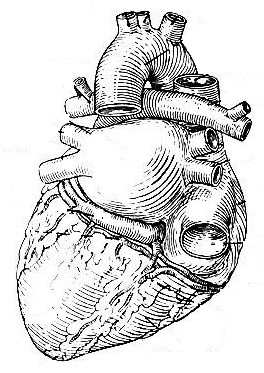
\includegraphics[width=2cm]{quiz/heartC.jpg}
 \choice 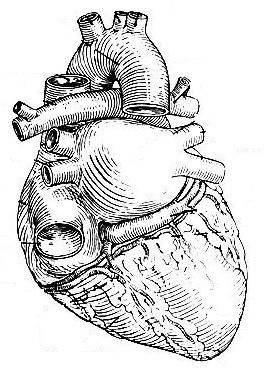
\includegraphics[width=2cm]{quiz/heartD.jpg}
\end{oneparchoices}
\hspace{1cm}
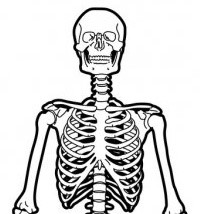
\includegraphics[]{quiz/skeleton.jpg}

\question The heart-beat (the sound you hear or feel when taking your pulse) is made by which of the following?
\begin{choices}
 \choice Contraction of the heart muscle
 \choice Emptying of the veins
 \choice Closing of the heart valves
 \choice Draining of the arteries
\end{choices}

\begin{multicols}{2}
\textit{Look at the picture of the heart, right and label the following. Each will only be used once.}
\question ``RIGHT VENTRICLE.''

\begin{oneparchoices}
 \choice A
 \choice B
 \choice C
 \choice D
\end{oneparchoices}
\question ``LEFT VENTRICLE.''

\begin{oneparchoices}
 \choice A
 \choice B
 \choice C
 \choice D
\end{oneparchoices}
\question ``RIGHT ATRIUM.''

\begin{oneparchoices}
 \choice A
 \choice B
 \choice C
 \choice D
\end{oneparchoices}
\question ``LEFT ATRIUM.''

\begin{oneparchoices}
 \choice A
 \choice B
 \choice C
 \choice D
\end{oneparchoices}
\columnbreak

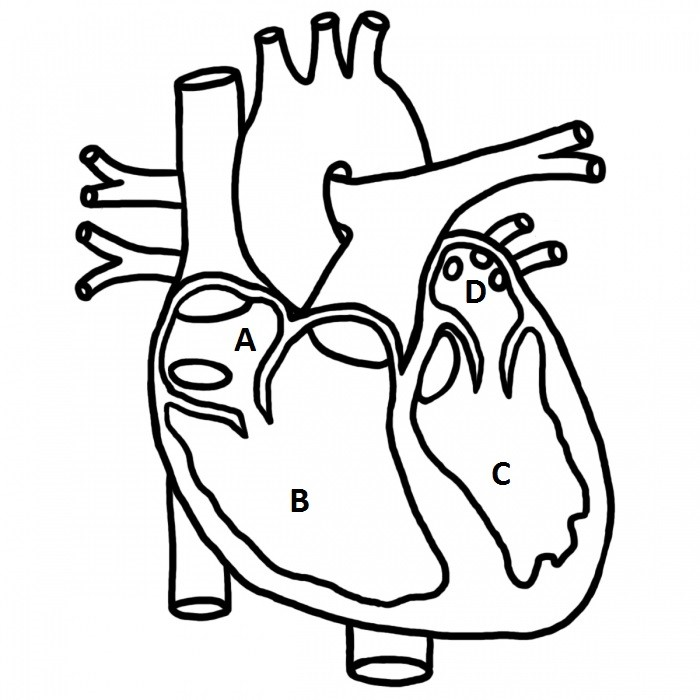
\includegraphics[width=0.3\textwidth]{quiz/heartmulti.jpg}
\end{multicols}

\question Two large veins drain blood from the upper body and lower body which empty into the \_\_\_\_\_ of the heart.
\begin{choices}
 \choice Left Atrium
 \choice Right Atrium
 \choice Left Ventricle
 \choice Right Ventricle
\end{choices}

\question Which part of the heart has thicker heart muscle:  The atria or ventricles?
\begin{choices}
 \choice Atria
 \choice Ventricles
\end{choices}

\begin{multicols}{2}
\question Look at the following heart, right.  Where does the blood go from this arrow?
\begin{choices}
 \choice It gets pushed into the atrium to be oxygenated by the lungs.
 \choice It gets drained into the veins to be distributed to the body.
 \choice It gets pushed into the aorta to be distributed to the body.
 \choice It gets drained into the other ventricle.
\end{choices}
\columnbreak

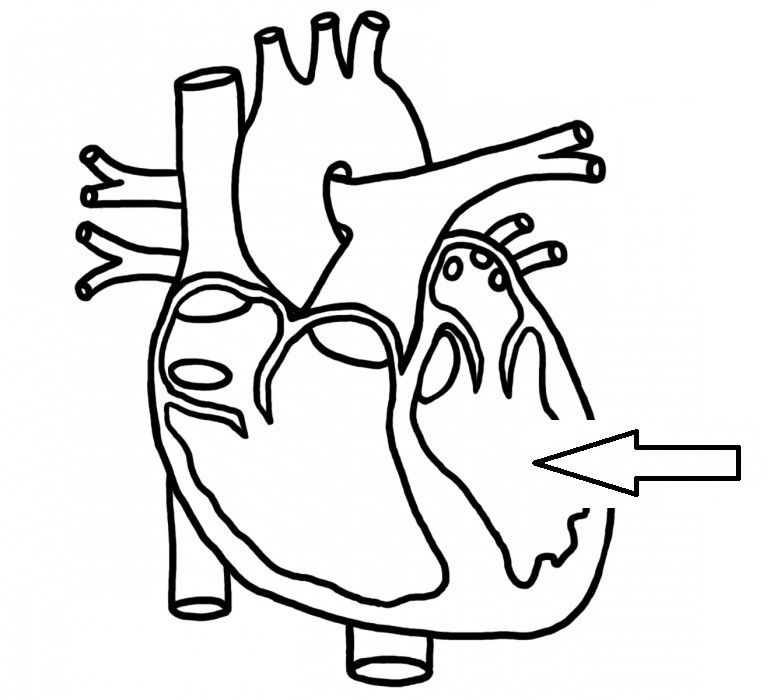
\includegraphics[width=0.3\textwidth]{quiz/heart10.jpg}

\end{multicols}

\begin{multicols}{2}
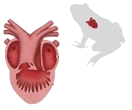
\includegraphics[width=0.3\textwidth]{quiz/frog.png}
\columnbreak

\question \textit{The Amphibian heart from a frog, is shown here, left.} \\ What is the consequence of having 1 fewer chamber as compared to the human heart?
\begin{choices}
 \choice Oxygen rich and oxygen poor blood mix in the ventricle.
 \choice The heart does not contract with as much force.
 \choice The lungs are not as effective in oxygenating blood.
 \choice The atria leak blood back into the ventricle.
\end{choices}
\end{multicols}

\begin{multicols}{2}
\question \textit{Look at the picture of the heart, right.} \\ Where do the lungs attach to the heart?
\begin{choices}
 \choice It gets pushed into the atrium to be oxygenated by the lungs.
 \choice It gets drained into the veins to be distributed to the body.
 \choice It gets pushed into the aorta to be distributed to the body.
 \choice It gets drained into the other ventricle.
\end{choices}
\columnbreak

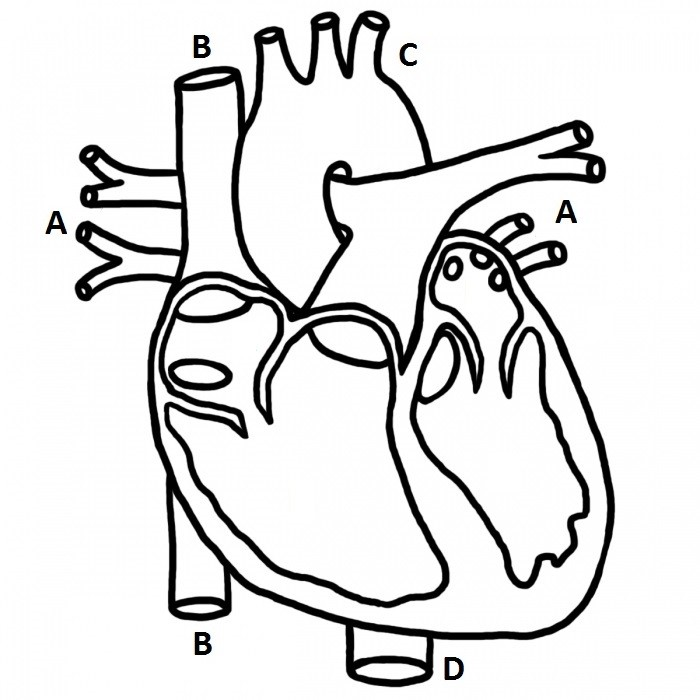
\includegraphics[width=0.3\textwidth]{quiz/heart12.jpg}

\end{multicols}

\begin{multicols}{2}
\question \textit{Please look at the cross-section of the heart, right, to answer the following question.  } \\ What would happen if this aortic valve (shown with an arrow) that separates the left ventricle from the aorta did not close?
\begin{choices}
 \choice Blood would flow back into the left ventricle.
 \choice Blood would flow into the aorta.
 \choice Blood would leak into the left ventricle.
 \choice Blood wouldn’t be pushed into the aorta.
\end{choices}
\columnbreak

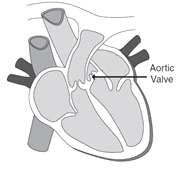
\includegraphics[width=0.3\textwidth]{quiz/heart13.png}

\end{multicols}
\end{questions}
\clearpage

\textbf{Answer Key:}
\begin{table}[!hbp]
\begin{tblr}{|X[c]|X[c]|X[c]|X[c]|X[c]|X[c]|X[c]|X[c]|}
\hline
\textbf{1 - D} & \textbf{2 - A} & \textbf{3 - C} & \textbf{4 - B} & \textbf{5 - C} & \textbf{6 - D} & \textbf{7 - A} & \textbf{8 - B} \\ \hline
\textbf{9 - B} & \textbf{10 - C} & \textbf{11 - A} & \textbf{12 - A} & \textbf{13 - C} & \SetCell[c=3]{black} & & \\ \hline
\end{tblr}
\end{table}

\end{document}